\section{Mathematical Background}

In this section we shall elaborate on the mathematical formulations and conceptual foundations upon which we aim to build this novel approach towards Topological Graph Theory with some unique data modelling characteristics. This section will also contain all corresponding references to the latest and most relevant research in the respective fields of Topology \& Graph Theory \& Topological Data Analysis. 

\subsection{Eulerian Graph Theory \& the Birth of Topology}


Graph theory is a well-established and versatile branch of mathematics that is primarily concerned with networks of points connected by lines. The subject of graph theory had its beginnings in recreational mathematical problems in the early 17th century, especially those related to the historical drawing of graphs stemming from cartographic representation of geographic regions. \cite{01.10_2001HistoryofGT} However, it has currently grown into a significant area of mathematical research, with applications in Chemistry, Biology, Operations Research, Social Sciences, Computer Science, Natural language processing \cite{22.0_2015_NLPGraphs} and Big-Data Analytics.\cite{22.1_BigDataPredictionGT} \cite{22.2_GTapplicationBigData} The history of graph theory may be specifically traced to 1735, when its founding father, Swiss Mathematician Leonhard Euler solved the Königsberg bridge problem. \cite{01.13_GTBackground}The Königsberg bridge problem was an old puzzle concerning the possibility of finding a path over every one of seven bridges that span a forked river flowing past an island—but without crossing any bridge twice. Euler argued that no such path exists. His proof involved only references to the physical arrangement of the bridges, but essentially he proved the first theorem in graph theory.\cite{01.11_1999historyofTopo}

\begin{figure}[H]
	\centering
	\includegraphics[width=\linewidth]{01_seven bridges of konigsberg.jpg}
	\caption{\textit{The above diagram shows the Königsberg bridge problem and its corresponding resolution by Leonhard Euler that lead to the introduction of graph theory and the subsequent birth of the branch of mathematical topology}}
	\label{fig:fig1}
\end{figure}

It is important to note, that in the field of Graph Theory, the term \textit{"graph"} does not refer to data charts, such as the likes of line graphs or bar graphs pertaining to the graphical visualization of data. Instead, it refers to a set of Vertices (V) (i.e., points or nodes) and Edges (E) (or lines) that connect the vertices. When any two vertices are joined by more than one edge, then such a graph is called a \textit{"Multi-graph"}. \cite{01.14_HDMultigraphs}\cite{01.13_GTBackground} A graph without any loops and with a maximum of one edge between any two vertices is called a \textit{simple graph}. When each and every vertex of a graph is connected by an edge to every other vertex, then such a  graph is called a \textit{complete graph}. Moreover, it is important to note in the context of this paper, a direction is assigned to each edge of a graph to produce what is known as a \textit{Directed Graph or Digraph}.\cite{20.0_2013AlgebraOfDAGs} We shall be dealing with such Directed Graphs for the remaining part of this paper.

Another useful concept in Graph Theory that of the \textit{path}. In this field, a path is defined as any route along the edges of a graph.\cite{01.13_GTBackground} A path may follow a single edge directly between two vertices, or it may follow multiple edges through multiple vertices.\cite{01.6_GTIntro} If there is a path linking any two vertices in a graph, then such a graph is called a \textit{connected graph}. A path that begins and ends at the same vertex without traversing any edge more than once is called a circuit, or a closed path. A circuit that follows each edge exactly once while visiting every vertex is known as an Eulerian circuit, and the graph is called an Eulerian graph. An Eulerian graph is connected and, in addition, all its vertices have even degree.\cite{01.16_EulerianGraphs} \cite{01.17_EulerianGraphOrientations} Such Eulerian Graphs shall be taken into consideration in the computational framework of our novel approach.

It is also important to know that the histories of graph theory and topology are closely related, and the two areas share many common problems and techniques even today, \cite{01.12_2013TopoHistHandbook} \cite{01.10_2001HistoryofGT} especially in the domains of mathematics and computer science. Such similarities can be traced back to Euler, who referred to his work on the Königsberg bridge problem as an example of \textit{geometria situs} or the “geometry of position”; while on the other hand, the development of topological ideas during  the 19th century became famously known as \textit{analysis situs}, or the “analysis of position” thereby interlinking these two fundamental pillars of mathematics.\cite{01.13_GTBackground}\cite{01.14_HDMultigraphs} As a further extension to the foundation of GT in 1750, Euler discovered the polyhedral formula $V - E + F = 2$ relating the number of \textit{vertices (V), edges (E), and faces (F)} of a polyhedron (a solid object in 3D geometry with each enclosed surface or face represented by polygons). \cite{01.12_2013TopoHistHandbook}\cite{01.16_EulerianGraphs}

The vertices and edges of all such polyhedrons form graphs on its surface, and this notion led to consideration of graphs on other surfaces such as a torus (the surface of a solid doughnut) and how they divide the surface into disk-like faces. Euler’s formula was soon generalized to surfaces as $V-E+F=2-2g$, where g denotes the genus, or number of “doughnut holes,” which help determine their Euler Characteristic. \cite{01.18_EulerFormula} Having considered a surface divided into polygons by an embedded graph, mathematicians began to study ways of constructing surfaces, and later more general spaces, by pasting polygons together. This was the beginning of the field of Combinatorial Topology, which later, through the work of the French mathematician Henri Poincaré and others, grew into what is known as Algebraic Topology.  \cite{01.1_1stCourse2018algebraicTopo} \cite{01.11_1999historyofTopo} \cite{01.12_2013TopoHistHandbook}Such concepts related to polyhedrons and Euler Characteristics that link the concepts of Graph Theory and Algebraic Topology through Combinatorics, serve as the theoretical basis for the mathematical formulations of our approach.

\subsection{Topological Data Analytics}

Topological Data Analytics or TDA \cite{02.3_2017introductionTDA} \cite{01_GCarlssonEpstein2011} is a mathematical methodology that is often represented as a useful computational framework or tool for high-dimensional data (i.e. data with multiple independent columns, variables or features across different datasets) analysis developed initially by Herbert Edelsbrunner, Afra Zomorodian, Gunnar Carlsson, and his graduate student Gurjeet Singh.\cite{01.9_2007MapperPBG} \cite{02.1_GCarlson2004topoEstimation} \cite{01_GCarlssonEpstein2011}The core idea of TDA  is based on the founding principle of Gunnar Carlson et.al\cite{02.4_TDAResearch} which states that, high-dimensional \& complex data sets (with multiple features and parameters) have intrinsic topological shape that can be represented in n-dimensions using generalized coordinate systems.\cite{01_GCarlssonEpstein2011} However, such shapes can then be assigned extrinsic characteristics and context-based meaning, thus enabling a robust and scalable framework of data labelling, classification and analysis. Such computational frameworks of topological analysis can be further enhanced and automated using Machine Learning and Neural Networks as elaborated in the later sections of this paper.the first data analysis framework using TDA was popularized by Carlsson’s paper in 2009  called \say{Topology $\&$ Data} \cite{02_carlsson2009topology} that later turned TDA into a hot field in applied mathematics, and also found many applications in Data-Science and Big-data Analytics.\cite{02.6_2009TDAChallenges}\cite{18.2_2018TDAonBigData} \cite{17.1_2012foundationsTGT} However, the mathematical foundations that drive TDA had been laid years before by others in the fields of Topology, Group Theory, Linear Algebra and Graph Theory as discussed earlier and referenced in this paper.


As evident today, an important feature of modern science and engineering is that data of various kinds is being produced at an unprecedented rate. \cite{02.6_2009TDAChallenges} \cite{18.2_2018TDAonBigData} This partly because of new experimental methods, and in partly because of the increase in the availability of high powered computing technologies.\cite{18.0_2016topologicalBigChem} \cite{18.1_2017TopoBigdataPipeline} It is also clear that the nature of the data that we obtain today is significantly different. For example, it is now often the case that we are given data in the form of very long vectors, where all but a few of the coordinates turn out to be irrelevant to the questions of interest, and further that we don't necessarily know which coordinates are the most relevant ones for the ideal solution. A related fact is that the data is often very high-dimensional, which severely restricts our ability to visualize it. The data obtained is also often much noisier than in the past and has more missing information (missing data).\cite{02_carlsson2009topology}

This is particularly so in the case of scentific data related to high throughput data \cite{11.0_chazal2017TopoDataScience}from micro-arrays in biology or other sources such as particle accelerators in high-energy physics, or in the case of multi-messenger data-streams in modern-day Astronomy. thus our ability to analyse such data, both in terms of quantity and the nature of the data, is  clearly not keeping pace with the data being produced.\cite{18.2_2018TDAonBigData} In this paper, we will discuss how geometry and topology can be applied to make useful contributions to the analysis of various kinds of data. Our aim is to establish that geometry and topology are very natural tools to apply in this direction, since geometry can be regarded as the study of distance functions, and in any statistical data-analysis model, we often end up applying such distance functions on large finite sets of data. The mathematical formalism which has been developed thus far for incorporating geometric and topological techniques deals with point clouds, i.e. finite sets of points equipped with a distance function. It then adapts tools from the various branches of geometry to the study of point clouds. The point clouds are intended to be thought of as finite samples taken from a geometric object, perhaps with noise.\cite{01_GCarlssonEpstein2011} \cite{01.9_2007MapperPBG} \cite{01.3_2016TDANewOpportunities}

However, our novel approach is different from traditional methods of topological analysis using point cloud data, in that it is primarily \textit{"Event-Driven"} in its technique, which appeals to a limited but widely applicable sub-set of Topological Graph Analysis where in hierarchical relationships can be determined between various dependent and independent column attributes of a dataset and can be then connected to a contextual \textit{"Event" or "Entity"} based on the choice of a \textit{``Lens''}, which will be further explored in our work. In all cases under consideration related to our approach, the  characteristics features of a dataset are associated to a central static context known as an "Event-Node" with independent features and variables associated with such events mapped to it in separate attribute clusters. This gives rise to well-defined hierarchical feature based multi-graphs with nodes and directed edges which represent the \textit{"micro-states"} of an Event, while its \textit{"macro-state"} is determined by the overall topology of the R-K diagrams with distinctive macro features such as holes, voids, loops etc. which can be characterised with the help of  Betti-Numbers which are unique to different classifications determined by domain specific filters and ontological parameters.

Now we shall note some of the key problems that occur when applying traditional statistical \&  geometric methods to data analysis that we aim to address using our analytical framework and pipeline:

$\bullet$ \textbf{\textit{High-dependence on Qualitative Information:}} One important goal of Data Analysis at its core, is to allow the user to obtain knowledge about the data, i.e. to understand how it is organized on a large scale. For example, if we imagine that we are looking at a data set constructed somehow from diabetes patients, it would be important to develop the understanding that there are two types of the disease, namely the juvenile and adult onset forms.\cite{01_GCarlssonEpstein2011}\cite{02.1_GCarlson2004topoEstimation} Once that is established, one of course wants to develop quantitative methods for distinguishing them, but the first insight about the distinct forms of the disease is key which needs to be qualified in non-topological analytical frameworks, where as differences in topological signatures of data pertaining to such patients can enable automated segregation for easier understanding and classification.

$\bullet$\textbf{\textit{Metrics are not Theoretically Justified:}} In physics and Astronomy, the phenomena studied often support clean explanatory theories which tell one exactly what metric to use. In biological problems, on the other hand, this is much less clear. But in certain cases it is far from clear how much significance to attach to the actual data points and distances, particularly at large scales and in developing fields of research such as in the case of Gravitational Wave Astronomy (LIGO, Virgo , etc.). Thus Topological frameworks such as ours would allow for smooth and effective measures of noise reduction in a phase-space independent of any metric dependencies while retaining the vital information isometrically, even in the case of transformations such as projection or compression.

$\bullet$\textbf{\textit{Coordinates are not Natural:}} Although we often receive data in the form of vectors of real numbers. However, it is frequently the case (in physics, astronomy and various branches of modern science) that the coordinates, like the metrics mentioned above, are not natural in any sense.Therefore it is incorrect to restrict ourselves to studying properties of the data which depend on any particular choice of coordinates. Note that the variation of choices of coordinates does not require that the coordinate changes be rigid motions of Euclidean space. It is often a tacit assumption in the study of data that the coordinates carry intrinsic meaning, but this assumption is often unjustified \cite{01_GCarlssonEpstein2011} \cite{02.1_GCarlson2004topoEstimation} \cite{02_carlsson2009topology} and can be effectively addressed in frameworks involving Topological Graph Analysis.

$\bullet$\textbf{\textit{Summaries are more valuable than individual parameter choices:}} In traditional approaches so far, a popular method of clustering a point cloud is the so-called single linkage clustering,  in which a graph is constructed whose vertex set is the set of points in the cloud, and where two such points are connected by an edge if their distance is  $\ge$ $\epsilon$, where $\epsilon$ is a parameter. \cite{02_carlsson2009topology} \cite{02.6_2009TDAChallenges} Some work in clustering theory has been done in trying to determine the optimal choice of $\epsilon$, but it is now well understood that it is much more informative to maintain the entire \textit{"Dendogram"} \cite{20.1_2001DAGMechanics}\cite{20.0_2013AlgebraOfDAGs} of the set, which provides a summary of the
behaviour of clustering under all possible values of the parameter  at once. It is therefore productive to develop other mechanisms in which the behaviour of invariants or construction under a change of parameters can be effectively summarized such as in the case of our novel framework.

\textit{We shall now discuss how Topological Graph Analysis could serve as an important and relevant way for addressing all the above mentioned problems especially to understand how they may be relevant in the case of formulating and justifying this novel approach for specific Analysis on Scientific and Ontology driven datasets that can be used to build useful Knowledge-Graphs and subsequent R-K Diagrams :}

\textbf{(1)} Topology and Graph theory are the best candidates in the branch of Analytics to deal with qualitative geometric information. This includes the study of what the connected components of a space are, but more generally it is the study of connectivity information, which includes the classification of micro-geometric properties such as nodes, edges and directions of DAGs \cite{20.0_2013AlgebraOfDAGs} to signify micro-state differences. While, macro-geometric properties are distinguished based on holes, voids, loops and higher dimensional surfaces within the space which are represented by distinct Euler Characteristics and Betti Numbers \cite{01.16_EulerianGraphs} \cite{01.17_EulerianGraphOrientations} of the specific unique topology. This suggests that extensions of topological \& graph methodologies, such as DAGs, Euler Characteristics, Betti Numbers, Homotopy \& Homology, should be helpful in studying them qualitatively.\cite{03.1_2009simplicialHomotopy} \cite{03_1944Homology}

\textbf{(2)} Topology \& Graph Theory study geometric properties in a way which is much less sensitive to the actual choice of metrics than straightforward geometric methods, which involve sensitive geometric properties such as curvature. \cite{01.1_1stCourse2018algebraicTopo} In fact, topology ignores the quantitative values of the distance functions and replaces them with the notion of infinite nearness of a point to a subset in the underlying space. This insensitivity to the metric is useful in studying situations where one only believes one understands the metric in a coarse way.\cite{02.3_2017introductionTDA}

\textbf{(3)} Topology studies only properties of geometric objects which do not depend on the chosen coordinates, but rather on intrinsic geometric properties of the objects. Therefore it allows for a  coordinate-free analytical approach. \cite{01_GCarlssonEpstein2011} \cite{02_carlsson2009topology}

\textbf{(4)} The idea of constructing summaries over whole domains of parameter values involves understanding the relationship between geometric objects constructed from data using various parameter values. The relationships which are useful involve continuous maps between the different geometric objects, and therefore become a manifestation of the notion of Functoriality, i.e,  the notion that invariants should be related not just to objects being studied, but also to the maps between these objects.\cite{05_mac2013Functoriality} Functoriality is central in algebraic topology in that the functoriality of homological invariants \cite{06.1_carlsson2008persistentHomo}is what permits one to compute them from local information, and that functoriality is at the heart of most of the interesting applications within mathematics. Moreover, it is understood that most of the information about topological spaces can be obtained through diagrams of discrete sets, via a process of simplicial approximation.\cite{03.1_2009simplicialHomotopy} \cite{08.2_1992simplicialAlgebricTopo}

\subsection{Topological Graph Theory}
The connection between graph theory and topology led to a sub-field called Topological Graph Theory.\cite{17.0_2001TGTIntro} \cite{17.1_2012foundationsTGT} An important problem in this area concerns planar graphs. These are graphs that can be drawn as dot-and-line diagrams on a plane (or, equivalently, on a sphere) without any edges crossing except at the vertices where they meet. Complete graphs with four or fewer vertices are planar, but complete graphs with five vertices or more are not. The use of diagrams of dots and lines to represent graphs actually grew out of 19th-century chemistry, where lettered vertices denoted individual atoms and connecting lines denoted chemical bonds (with degree corresponding to valence), in which planarity had important chemical consequences. The first use, in this context, of the word graph is attributed to the 19th-century Englishman James Sylvester, one of several mathematicians interested in counting special types of diagrams representing molecules.\cite{17.2_TGTonlineBritanica}

Topological graph theory deals with ways to represent the geometric realization of graphs. Typically, this involves starting with a graph and depicting
it on various types of drawing boards: 3-space, the plane, surfaces, books,
etc. This field mainly uses topological methods to study graphs. For example, planar graphs
have many special properties. The field also uses graphs to study topology.
For example, the graph theoretic proofs of the Jordan Curve Theorem, or
the theory of voltage graphs depicting branched coverings of surfaces, provide an intuitively appealing and easily checked combinatorial interpretation
of subtle topological concepts \cite{17.3_1996topologicalGT} \cite{17.1_2012foundationsTGT} that serve as the fundamental basis of this novel approach and are establish as a part of our computational framework. 

\subsubsection{Directed Acyclic Graphs}
In our paper, we enable a topological graph theory framework through DAG's at the micro level which can be defined as follows:

A directed acyclic graph is a graph $(N,E) \in G$ where $G$ is a graph $N$ are nodes and $E$ are edges. It is a restricted general graph, in that there are no edge cycles, such that an edge can be described as $E_{N_i,N_j}$ where $i \ne j$ and the path of edges never roll back onto itself. The benefit of a DAG is the composibility of it, and the ability to make complicated and general pipelines from it.

\subsection{Phase Space \& Projections}
In the last century, the development of modern physics has been partially driven by the incorporation of a few key concepts. A phase space is the spatial representation of all possible states of a dynamical system, where each point uniquely identifies a state. A Topological Phase Space can be defined as the n-dimensional spatial representation of the same using a generalized Curvilinear Coordinate system allowing for all possible coordinate transformations and perfect isometric compressions while preserving geometric invariance.
The concept of Phase Space in itself is a simple but powerful idea that emerged in the second half of the 19th century, during the golden era of differential geometry, and it is at the core of modern classical, quantum, and statistical mechanics. The trajectory that a dynamical system describes in the phase space as it evolves with time contains rich information about the system. For instance, by looking at the shape of the trajectories that a pendulum describes in its phase space, we can infer the existence of different dynamical regimes, or the ratio between the length of the pendulum and the acceleration of gravity.

\begin{figure}[H]
	\centering
	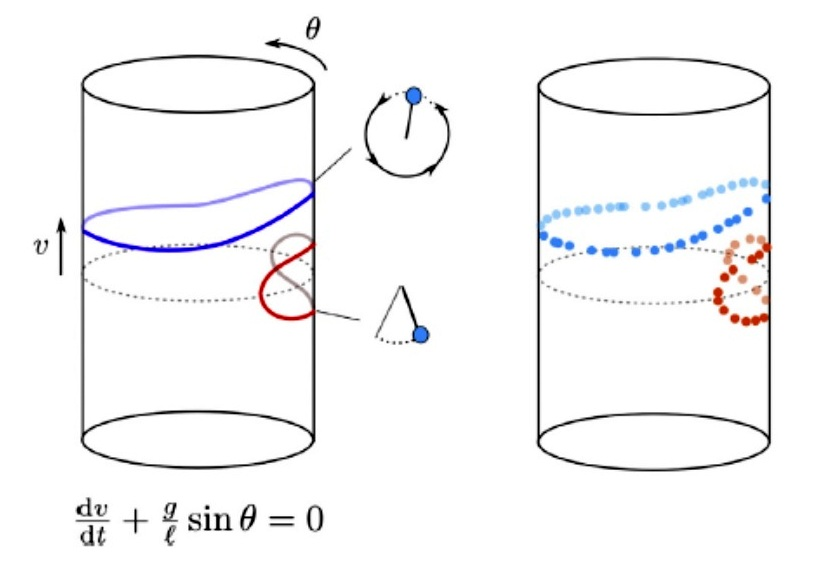
\includegraphics[width=\linewidth]{03_Phase Space Projections.jpg}
	\caption{\textit{the above diagram shows that the phase space of a simple pendulum is a two-dimensional cylinder, where the periodic coordinate corresponds to the angle  of the pendulum with respect to the vertical, and the longitudinal coordinate to its angular velocity}}
	\label{fig:fig2}
\end{figure}

Each point in this space specifies a unique combination of the position and velocity and uniquely determines the subsequent evolution. For small angular velocities, the pendulum oscillates back and forth around the equilibrium point. For large velocities, the pendulum describes a circular motion.

\subsection{Homotopy \& Homology}

\textbf{Homotopy} \cite{03.1_2009simplicialHomotopy} \cite{08.1_2003SimplicialHomology} is defined as  a continuous deformation of one continuous function $f(x)$ to another continuous function $g(x)$ without break in topology from shearing and  tearing resulting in discontinuities or the formation of holes or gluing resulting from merger of holes that would also result in discontinuous functions. This gives rise to the notion of “essential-sameness” whereby one geometric shape can be continuously deformed into any other without tearing or shearing just like a doughnut can be converted to a mug with one whole via a smooth transformation with continuous deformations. Conversely, the doughnut cannot be converted into a sphere without gluing in terms of merging the space in between and hence such geometric shapes can be considered “essentially-different” as they cannot be inter-converted into smooth functions via continuous deformations as shown in the figure below.\cite{07_bjorner2003Homotopy}

\begin{figure}[H]
	\centering
	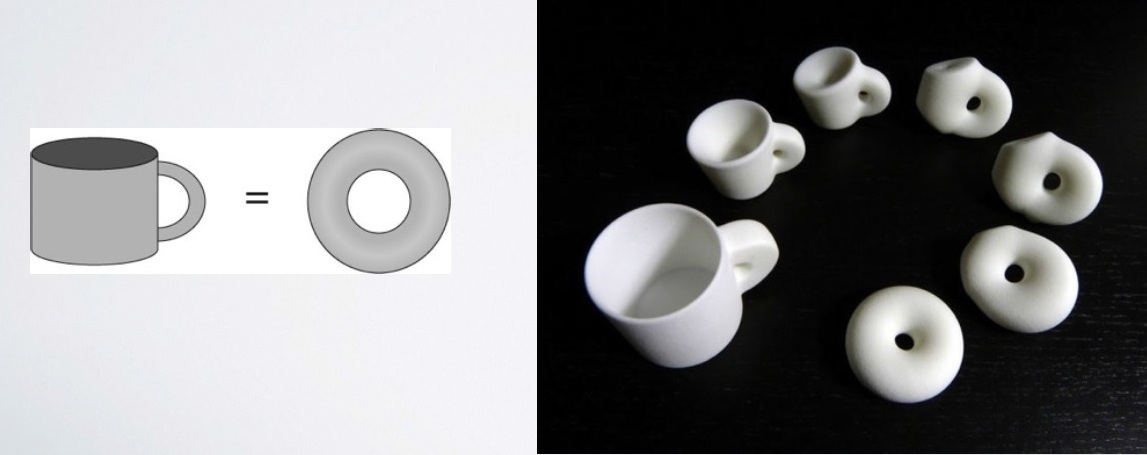
\includegraphics[width=\linewidth]{02_Homotopy cup doughnut.jpg}
	\caption{\textit{the above figure shows how the geometric shape of a cup $f(x)$ can be smoothly transformed into that of a doughnut $g(x)$ using continuous deformations without any discontinuities or break in topology resulting from tearing, shearing or gluing as both geometric figures begin and end with 1 hole and thus abide by the notion of “essential-sameness” in Topology. }}
	\label{fig:Homotopy}
\end{figure}

We can describe the formalism in more standard mathematical terms as follows: From the above definition and description, we can say that two continuous maps $f, g : X \rightarrow Y$ are said to be \say{Homotopic} if there is a continuous map  $H :X \times [0, 1] \rightarrow Y$ such that $H(x, 0) = f(x)$ and $H(x, 1) = g(x)$. We also say that a map $f : X \rightarrow Y$ is a homotopy equivalence if there is a map $G : Y \rightarrow X$ so that $f \circ g$ is homotopic to the identity map on Y and $g \circ f$ is homotopic to $f$. Two spaces $X$ and $Y$ for which there exists a homotopy equivalence $f : X \rightarrow Y$ are said to be homotopy equivalent. A space that is homotopy equivalent to the one point space is said to be \textit{contractible}. \cite{07.1_Homotopy} \cite{07_bjorner2003Homotopy}

\textbf{\textit{Definition:}} Thus we can conclude that for any topological space $X$, in Abelian group $A$, with integer $j \ge 0$, there is assigned a group $H_j(X,A)$ which defines the Homotopy.

\textbf{\textit{Functoriality:}} For any A and j as above, and any continuous map $f : X \rightarrow Y$, there is an induced homomorphism $H_j(f,A) : H_j(X,A) \rightarrow H_j(Y,A)$. Therefore, one has $H_j(f \circ g,A) = H_j(f,A) \circ H_j(g,A)$ and $H_j(Id_X;A) = Id_(Hk(X,A))$.These conditions are called collectively \textit{functoriality}.\cite{05_mac2013Functoriality}

\textbf{\textit{Homotopy invariance:}} If $f$ and $g$ are homotopic, then $H_j(f,A)=H_j(g,A)$. It follows that if $X$ and $Y$ are homotopy equivalent, then $H_j(X,A)$ is isomorphic to $H_j(Y,A)$.\cite{01.0_2010introductionTopoPropertiesInvariance} \cite{12.0_alatorre2018TDAinvariant}

\textbf{\textit{Normalization:}}$H_0(\star,A) \approx A$, where $\star$ denotes the one point space.

\textbf{\textit{Betti numbers:}} For any field F, $H_j(X, F)$ will be a vector space over $F$. Its dimension, if finite, will be written as $\beta_j(X, F)$, and will be referred to as the j-th Betti number with coefficients in F. The j-th Betti number corresponds to an informal notion of the number of independent j-dimensional surfaces. If two spaces are homotopy equivalent, then all their Betti numbers are equal with the following properties:

Property 1: For any topological space $X$ with a finite number of path components, $\beta_0(X)$ is the number of path components.

Property 2:  If the first Betti number $\beta_1$ of the letter “B” above is two, and for the letter “A” it is one, for any field $F$, then in this case, it provides a formalization of the count of the number of loops present in the space. \cite{07.2_TopoBettiNumbers} \cite{02_carlsson2009topology}

\textbf{\textit{Homology}}  is defined as a concept in algebraic topology that provides a  powerful tool to formalize and handle the notion of topological features of a topological space or of a simplicial complex in an algebraic way. For any dimension $j$, the $j-dimensional$ “holes” are represented by a vector space $H_j$ whose dimension is intuitively the number of such independent features. For example the 0-dimensional homology group $H_0$ represents the connected components of the complex, the 1-dimensional homology group $H_1$ represents the 1-dimensional loops, the 2-dimensional homology group $H_2$ represents the 2-dimensional cavities and so on.\cite{03.2_2008FindingHomology} \cite{03.3_de2007PersistentHomology} \cite{03.4_2008localizedHomology}


\subsection{Euler Characteristics \& Betti Numbers}

The Euler Characteristic is a useful tool in mathematics that is used to classify topological characteristics of various classes of polyhedrons, based only on a relationship between the numbers of vertices (V), edges (E), and faces (F) of any geometric figure.\cite{07.2_TopoBettiNumbers}

Mathematically, it can be defined as a number $X$, such that: $X = V - E + F$ where $V, E \& F$ represents the number of Vertices, Edges $\&$ Faces of the polyhedron respectively. The Euler Characteristic can also be represented as: $X =2(1-g)$ where  $g= X/2-1$ is known as the genus  of the polyhedron \cite{17.2_TGTonlineBritanica} which can be understood intuitively as the “number of holes” in the polyhedron or geometric figure. The genus theorem states for a polyhedron embedded on an orientable closed surface − or the corresponding combinatorial orientated map −, the Euler characteristic  $X = V − E + F$ is always an even integer, possibly negative, and that, c being the number of connected components of the polyhedron, its genus $g = c − \chi/2$ is a natural number. In fact, g corresponds to the number of holes in the surface of the polyhedron. When g = 0, the surface is without holes, and the polyhedron is said to be planar. When it is also connected $(c = 0)$, it satisfies the Euler formula which is a special case of the Euler Characteristic, given by:  $V−E+F= 2$; for instance, in the case of a cube that has 8 vertices, 12 edges and 6 faces: $V−E + F=8-12+6=2$.\cite{03_1944Homology} \cite{01.18_EulerFormula}

However, our special concern for understanding the genus of a polyhedron is its relation to Betti Numbers and  Euler Characteristics in Topology. Betti numbers are topological objects which were proved to be invariants by Poincaré, and used by him to extend the polyhedral formula to higher dimensional spaces. Informally, the Betti number is the maximum number of cuts that can be made without dividing a surface into two separate pieces. Formally, the $n^{th}$ Betti number is the rank of the $n^{th}$ homology group of a topological space. Betti numbers can be related to Euler Characteristics of Polyhedrons and their genus via the following mathematical relation.\cite{03.7_2018homologicalAlgebra&Data} \cite{07.3_BettiNumber} \cite{07.2_TopoBettiNumbers}

\begin{equation}
  X=\sum_{n \ge 0}(−1)^{n}\beta_{n}(\sum)=2(c - g)
\end{equation}

where the $n^{th}$ dimensional Betti number $\beta_n$ is the dimension of the $n^{th}$ homology group $H_n(\sum)$ of the $SC \sum$. These are important metrics that would characterize the topology of the data and would be significant in various steps of our computational pipeline in the following sections.\cite{01.16_EulerianGraphs} \cite{01.18_EulerFormula} \cite{17.2_TGTonlineBritanica} \cite{03.2_2008FindingHomology} \cite{08.1_2003SimplicialHomology}


\subsection{Simplicial Complexes}
The concept of Simplicial Complexes \cite{03.1_2009simplicialHomotopy} \cite{08_1971simplicialComplex} are quite essential to Homology that applies to all topological spaces (singular homology) relies on the linear algebra of infinitely generated modules over the ring $Z$ in defining homology groups, and for this reason it is not useful from a computational point of view. Computations can be carried out by hand using a variety of techniques (long exact sequence of a pair, long exact Mayer-Vietoris sequence, excision theorem, spectral sequences), but direct computation from the definition is not feasible for general spaces.\cite{03.2_2008FindingHomology}
However, when one is given a space equipped with particular structures, there are often finite linear algebra problems which produce correct answers, i.e. answers which agree with the singular technique. A particularly nice example of this applies when the space in question is described as a “simplicial complex”.\cite{08.2_1992simplicialAlgebricTopo} \cite{08.3_2018simplicialComplexes}

\subsection{Persistent Homology}
Persistent homology \cite{03.3_de2007PersistentHomology} \cite{03_1944Homology} \cite{03.3_de2007PersistentHomology} can be explained as a method for computing stable topological features of a dataset through evaluating transformations over varying parameters, such as spatial resolutions against point cloud data. It gives a multi-scale view of the topology of a space by capturing the evolution of topology with increasing (or decreasing) resolutions. It  is a powerful tool to compute, study and encode efficiently multi-scale topological features of nested families of simplicial complexes and topological spaces. It not only provides efficient algorithms to compute the Betti numbers of each complex in the considered families, as required for homology inference in the previous section, but also encodes the evolution of the homology groups of the nested complexes across the scales.\cite{03.7_2018homologicalAlgebra&Data}
The input data for the computation of persistent homology is often represented as a point cloud. The output is a set of real number pairs (the birth and death times) documenting the spatial resolutions where each topological feature first appears (birth) and when it disappears (death). The pairs are usually plotted either as a set of lines, called bar-codes, as a set of points in a 2D plane, called a persistence diagram, or as a persistent landscape. Most implementations of the persistent homology are done over point cloud data via the Mapper algorithm \cite{01.9_2007MapperPBG}, however the core concept of persistent homology extends past it's traditional implementation on point cloud data in ways such as data related to knowledge graphs.\cite{01.1_1stCourse2018algebraicTopo}\cite{03.2_2008FindingHomology}

\textbf{\textit{Example:}}  We shall now consider a typical example of how Persistent  Homology has been implemented thus far in the domain of Topological Data Analytics. So, in order to demonstrate the concept of  persistent homology, let us imagine we have collected a bunch of data points that we refer to as a data cloud. For the next step, let us imagine that there is a control parameter called the proximity parameter $\epsilon$, which defines the radius of an imaginary ball centered at each of these data points.\cite{01_GCarlssonEpstein2011} \cite{02.1_GCarlson2004topoEstimation}\cite{03.6_2015persistentHomo}

Now, when we gradually increase $\epsilon$, the balls will grow outwards and eventually touch other balls. The overlapping of these balls form a unique topological characteristic that is unique to this dataset, and hence we can use this unique topological characteristic to differentiate nuances in the topologies of different point clouds. This filtration process can be demonstrated and visualized in the figure below:\cite{06.2_carlsson2009Multipersistence}

\begin{figure}[H]
	\centering
        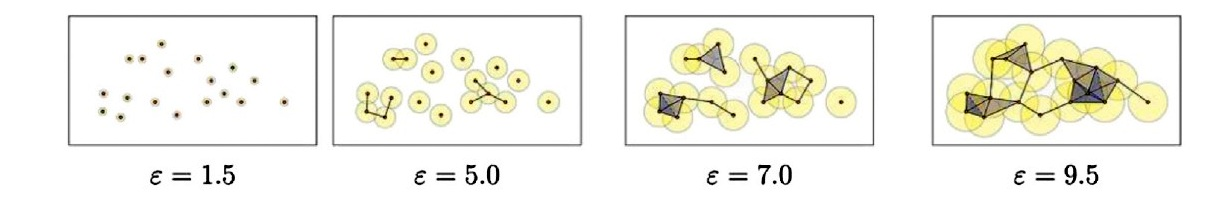
\includegraphics[width=1.0\linewidth]{images/Persitent Homology Point Cloud Filtration Process.jpg}
	\caption{\textit{The figure above shows a schematic diagram representing a data cloud, and how the filtration process results in outcomes of various overlapping of balls from different proximity parameters $\epsilon$ (shown in the upper column). The bottom column is barcodes scanning through a full-range of proximity parameter $\epsilon$ values. $\beta_0$ and  $\beta_1$ denote the 0-dimensional and 1-dimensional Betti numbers, which can be deduced from the subfigures to be roughly $18\rightarrow11\rightarrow4\rightarrow1$, and $0\rightarrow0\rightarrow1\rightarrow2$, respectively.}}
	\label{fig:example_pipeline_fig}
\end{figure}

Thus standard practices in TDA use a similar  encoding and filtration process, as shown above to convert a point cloud that is made from brain functional signals, or a correlation matrix from examples such as time series data, to filtration diagrams. From these filtration diagrams, we can calculate barcodes, persistence diagrams, and other TDA metrics for further applications of Persistent Homology.\cite{03.4_2008localizedHomology}\cite{03.3_de2007PersistentHomology}

Thus, Persistent homology can be explained  as a method for computing topological features of a data set (point cloud) at different spatial resolutions. It gives a multi-scale view of the topology of a space by capturing the evolution of topology with increasing (or decreasing) resolutions. It  is a powerful tool to compute, study and encode efficiently multi-scale topological features of nested families of simplicial complexes and topological spaces. It not only provides efficient algorithms to compute the Betti numbers of each complex in the considered families, as required for homology inference in the previous section, but also encodes the evolution of the homology groups of the nested complexes across the scales.\cite{03.2_2008FindingHomology}\cite{03.3_de2007PersistentHomology}\cite{09.2_chazal2008CompGeometry} \cite{11.0_chazal2017TopoDataScience}

\subsection{Topological Projection \& Isometric Compression of Graphs}

The mathematics of projection\cite{12.1_2002topologicalInvariaceProjection} is defined in terms of a mapping of a set or other mathematical structures such as operations, metrics or topology into a subset (or sub-structure), which is equal to its square for mapping Function  Composition  which can be mathematically defined as a function $h(x)$ such that $h(x) = g(f(x))$ That is, the functions $f \: X \rightarrow Y$ and $g \: Y \rightarrow Z$ are composed to yield a function that maps x in X to $g(f(x))$ in Z.\cite{12.2_ProjectionMath}  Projections can be intuitively explained as casting a shadow of  geometric points or objects  on a plane or a sheet of paper. For example the shadow projection of a point on a plane or a sheet of paper is the point itself; whereas, the shadow projection of a 3-D sphere is a closed circle which is equal to the square of its mapping function and can be used to obtain the original topology of the 3-D sphere without the loss of essential information.\cite{12.0_alatorre2018TDAinvariant}

The mathematical appeal and utility of projection is that it's fundamentally elementary and geometric with a finite number of degrees of freedom; once the acceptance domain and the dimensions of the spaces used in the construction are chosen which allows for easier manipulation of higher dimensional data and applying essential filters and transformation in the domain of TDA. This also helps us to obtain all essential information from high-dimensional data sets while carrying out efficient noise reduction. It also preserves and amplifies the essential nature of such datasets for analysis and obtaining useful insights from its underlying attributes and relationships.\cite{01.0_2010introductionTopoPropertiesInvariance}\cite{02.3_2017introductionTDA} \cite{02.4_TDAResearch}

In the field of Topology, we mostly work with the special class of point sets obtained by cut and projection from the integer lattice $Z^{N}$ which is generated by an orthonormal base of $R^{N}$. In short we can call a projection method pattern $T$ on $E = R^{d}$ a pattern of points (or a finite orientation of it) given by the orthogonal projection onto E of points in a strip $(K × E) \cap Z^{N} \subset R^{N}$, where E is a subspace of $R^{N}$ and $K × E$ is the so-called acceptance strip, a flattening of $E$ in $R^{N}$ defined by some suitably chosen region K in the orthogonal complement $E \perp$ of $K$ in $R^{N}$. The pattern $T$ thus depends on the dimension N, while also depending on the positioning of E in $R^{N}$ and the shape of the acceptance domain K. When this construction was first made, the domain $K$ was taken to be the projected image onto $E \perp$ of the unit cube in $R^{N}$ and this choice gives rise to the so-called canonical projection method patterns in Topology and TDA that are useful concepts which are essential in establishing a feasible and seamless way to carry out near-lossless topological projections and isometric compression of data-structures represented by DAGs and multi-graphs in this novel approach.\cite{12.0_alatorre2018TDAinvariant} \cite{12.1_2002topologicalInvariaceProjection}

The application of isometric compression of graphs \cite{03.5_kramar2013persistenceComputing} \cite{12.2_compressingTopoNetworkGraphs} is further useful as the mathematics of Topology allows for unique possibilities that provide methods for creating compressed representations of data sets that retain all features of the original data set via efficient techniques such as Isometric Compression. These represent the various relationships among points in the data set. The representation is in the form of a topological network or combinatorial graph, which is a very simple and intuitive object to work with using graph layout algorithms and allows for the comparative analysis of all essential attributes of the original high-dimensional dataset without loss of essential information. This provides a unique and necessary advantage over standard graphical visualizations and data plots which only address and compare 2 or more limited subset of variables, dimensions or columns of the high-dimensional dataset.\cite{21.0_2016TopoCompression}
